\documentclass{article}
\usepackage{tikz}
\usetikzlibrary{arrows.meta}

\begin{document}

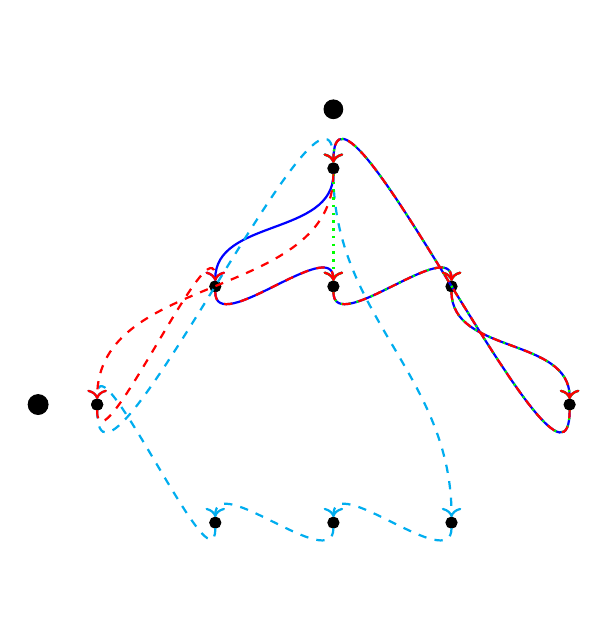
\begin{tikzpicture}[scale=1.5, every node/.style={circle, draw, fill=black, minimum size=4pt, inner sep=0pt, outer sep=0pt}]
    % Nodes
    \node (v) at (0, 2) {};
    \node (u) at (-2, 0) {};
    \node (w1) at (-1, 1) {};
    \node (w2) at (0, 1) {};
    \node (w3) at (1, 1) {};
    \node (w4) at (2, 0) {};
    \node (w5) at (1, -1) {};
    \node (w6) at (0, -1) {};
    \node (w7) at (-1, -1) {};
    \node (w8) at (-2, 0) {};

    % Edges
    \draw[blue, thick, ->] (v) to[out=-90,in=90] (w1);
    \draw[blue, thick, ->] (w1) to[out=-90,in=90] (w2);
    \draw[blue, thick, ->] (w2) to[out=-90,in=90] (w3);
    \draw[blue, thick, ->] (w3) to[out=-90,in=90] (w4);
    \draw[blue, thick, ->] (w4) to[out=-90,in=90] (v);

    \draw[dashed, cyan, thick, ->] (v) to[out=-90,in=90] (w5);
    \draw[dashed, cyan, thick, ->] (w5) to[out=-90,in=90] (w6);
    \draw[dashed, cyan, thick, ->] (w6) to[out=-90,in=90] (w7);
    \draw[dashed, cyan, thick, ->] (w7) to[out=-90,in=90] (w8);
    \draw[dashed, cyan, thick, ->] (w8) to[out=-90,in=90] (v);

    \draw[dotted, green, thick, ->] (v) to[out=-90,in=90] (w2);
    \draw[dotted, green, thick, ->] (w2) to[out=-90,in=90] (w3);
    \draw[dotted, green, thick, ->] (w3) to[out=-90,in=90] (w4);
    \draw[dotted, green, thick, ->] (w4) to[out=-90,in=90] (v);

    \draw[dashed, red, thick, ->] (v) to[out=-90,in=90] (u);
    \draw[dashed, red, thick, ->] (u) to[out=-90,in=90] (w1);
    \draw[dashed, red, thick, ->] (w1) to[out=-90,in=90] (w2);
    \draw[dashed, red, thick, ->] (w2) to[out=-90,in=90] (w3);
    \draw[dashed, red, thick, ->] (w3) to[out=-90,in=90] (w4);
    \draw[dashed, red, thick, ->] (w4) to[out=-90,in=90] (v);

    % Labels
    \node at (0, 2.5) {$v$};
    \node at (-2.5, 0) {$u$};

\end{tikzpicture}

\caption{A connected DFA with an $f$-corner $v$ and a $g$-corner $u$. Here, $f:\Psi^* \rightarrow \{-1,1\}$ is a function in which a word is positive if and only if it begins with red (dashed) or blue (solid), and $g:\Psi^* \rightarrow \{-1,1\}$ is a function in which a word is positive if and only if it does not begin with red (dashed).}
\end{document}